\section{Red hogare\~na}
Esta red en principio es muy controlada y solo sabemos que cuenta con un n'umero peque\~no de nodos. La red usa
en su mayoria wi-fi por lo cual es de esperar que el nodo que usamos para monitorear la red reciba amplia cantidad de
paquetes who-has y is-at dado que no hay switches segmentando la red que filtren respuestas is-at de terceros.

El primer experimento, el cual ve la red como una fuente con 2 simbolos unicamente, arroja luego de monitorear la red durante 30 minutos
que en ella  la mayor parte del trafico es unicast y solo el 17\% es broadcast.

\begin{tabular}{ r|c|c| }
\multicolumn{1}{r}{}
 &  \multicolumn{1}{c}{frecuencia}
 & \multicolumn{1}{c}{informaci'on} \\
\cline{2-3}
broadcast & 0.17 & 2.56 \\
\cline{2-3}
unicast & 0.83 & 0.27 \\
\cline{2-3}
\end{tabular}
 
 Estos valores nos dan una entropia de 0.66 bits (siendo el m'aximo 1 dado que hay 2 simbolos en principio equiprobables) lo
 cual concuerda con las expectativas dado que en una red local hogare\~na se espera ver mas que nada trafico unicast entre
 los nodos y el gateway hacia internet.
 
TODO TODO
 
\begin{figure}[!h]
\centering
\caption{xxxx}
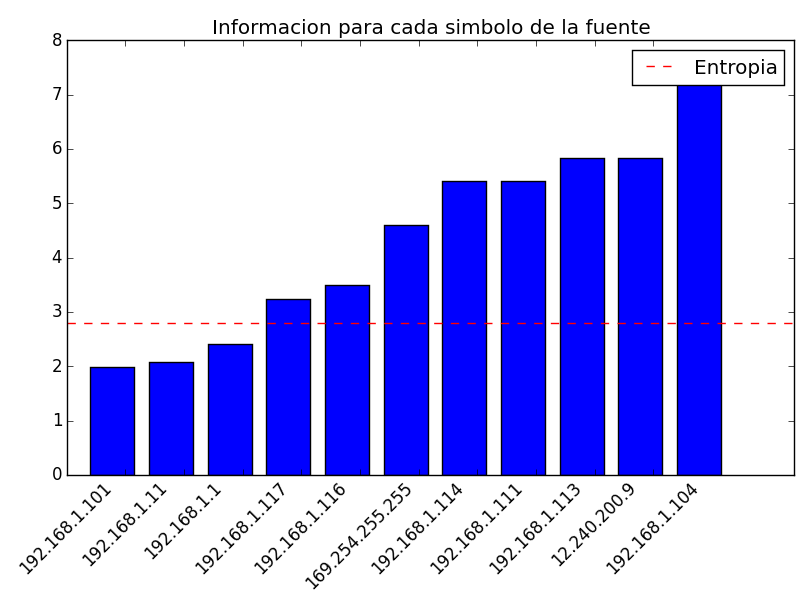
\includegraphics[width=0.55\textwidth]{red1_info}
 \label{fig:xxxx}
\end{figure}



\begin{figure}[!h]
\centering
\caption{xxxx}
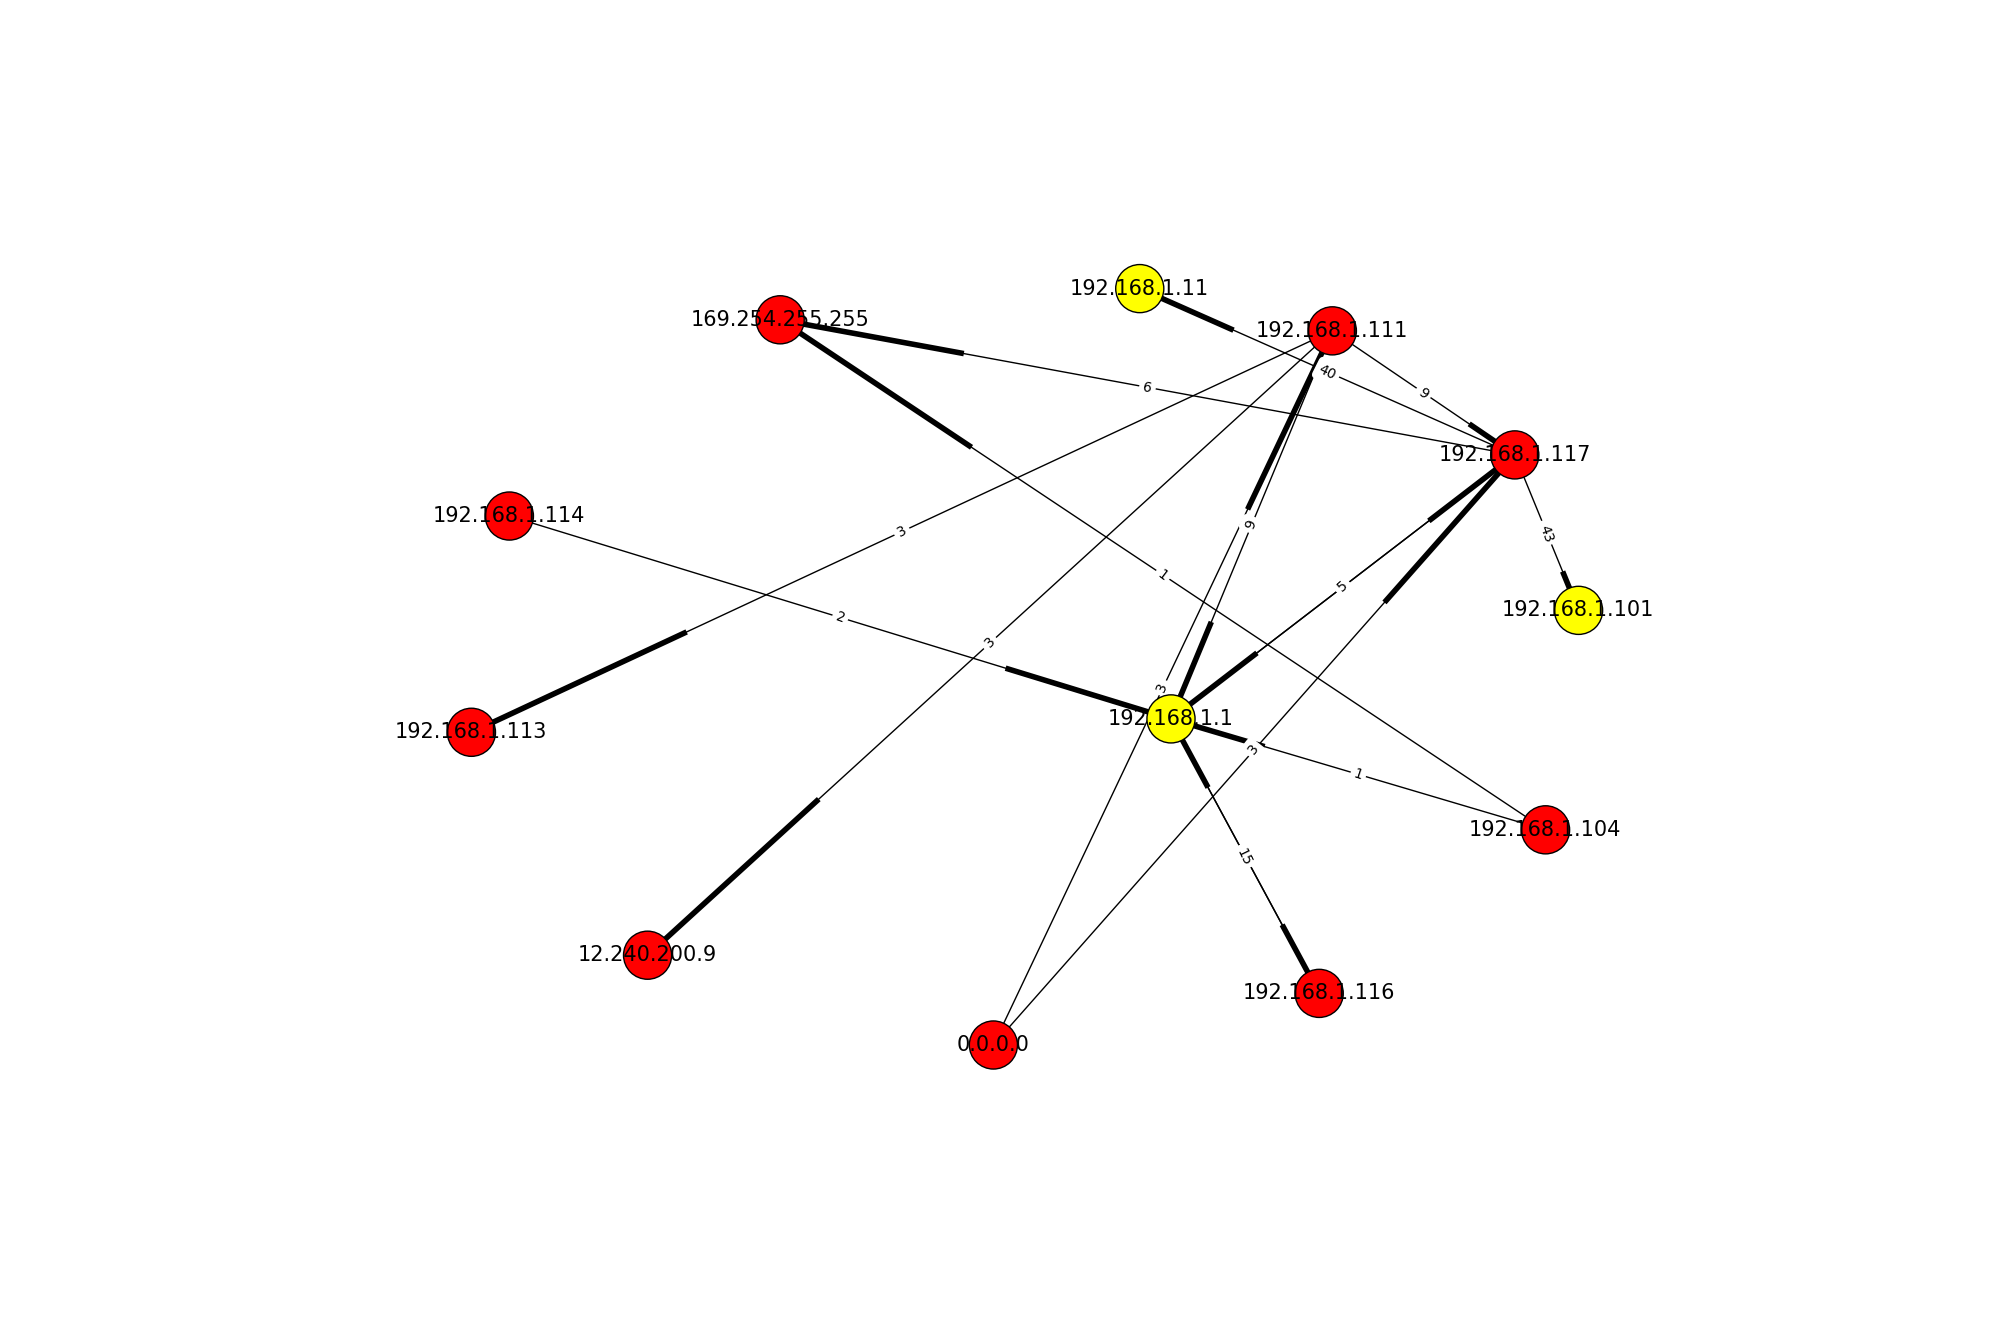
\includegraphics[width=0.85\textwidth]{red1_red}
 \label{fig:xxxx}
\end{figure}
